\documentclass[10pt,landscape]{exam}
\usepackage[phy]{template-for-exam}
\usepackage[margin=0.4in]{geometry}
\usepackage{multicol,silence,graphicx}

\WarningFilter{latex}{Label `question}
\WarningFilter{latex}{There were multiply-defined labels}
\WarningFilter{latex}{Label `part}
%%%%%%%%%%%%%%%%%%%%%%%%%%%%%%%%%%%%%

\def\todayDate{Wed, Sept 9 (Pd 6) / Fri, Sept 11 (Pd 1, 3) }

\def\content{

The girl in the picture throws the ball.  At point $A$, it leaves her had with a velocity of $+7$~m/s.  Right \emph{before} she catches it at point $C$, what is the ball's velocity?  Explain in a few complete sentences why this is the case.

\vspace{1em}

\noindent
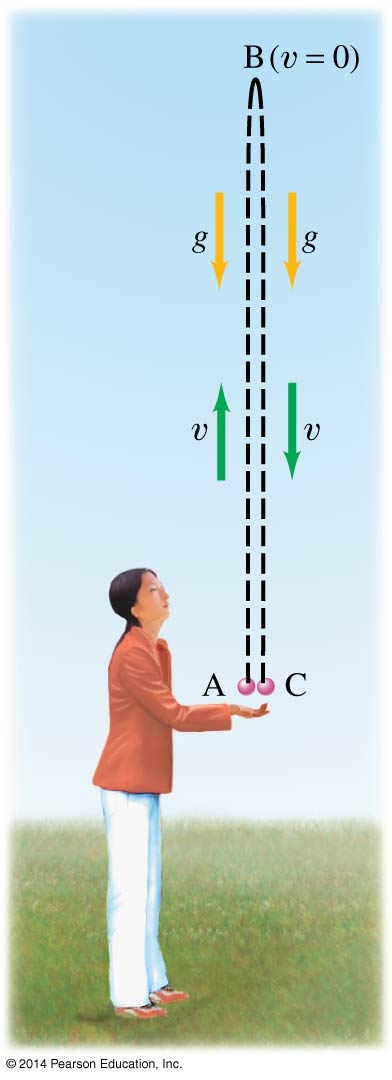
\includegraphics[height=10cm]{02_23_Figure.jpg}


\vspace{12em}

\noindent
{\footnotesize The image is Figure 2-23 from Giancolli \emph{Physics: Principles with Applications}, 7th edition.}

}

%%%%%%%%%%%%%%%%%%%%%%%%%%%%%%%%%%%%%%

\begin{document}
\pagestyle{empty}

\setlength{\columnsep}{0.8in}
\begin{multicols*}{2}

\noindent  
Name: \hfill Period: \hspace{5em}
\vspace{0.5em}
\hrule

\section*{\todayDate}
\subsection*{Warmup}

\content

\vfill
\hrule
\vspace{0.5em}
\hfill {\sc Physics I}

\columnbreak

\noindent  
Name: \hfill Period: \hspace{5em}
\vspace{0.5em}
\hrule

\section*{\todayDate}
\subsection*{Warmup}

\content

\vfill
\hrule
\vspace{0.5em}
\hfill {\sc Physics I}

\end{multicols*}

\end{document}